\documentclass[journal]{IEEEtran}
\usepackage{amsmath, amsfonts, graphicx, listings, xcolor, float, subfig}

\definecolor{codegreen}{rgb}{0,0.6,0}
\definecolor{codegray}{rgb}{0.5,0.5,0.5}
\definecolor{codepurple}{rgb}{0.58,0,0.82}
\definecolor{backcolour}{rgb}{0.95,0.95,0.92}

\lstdefinestyle{mystyle}{
    backgroundcolor=\color{backcolour},   
    commentstyle=\color{codegreen},
    keywordstyle=\color{magenta},
    numberstyle=\tiny\color{codegray},
    stringstyle=\color{codepurple},
    basicstyle=\ttfamily\footnotesize,
    breakatwhitespace=false,         
    breaklines=true,                 
    captionpos=b,                    
    keepspaces=true,                 
    numbers=left,                    
    numbersep=5pt,                  
    showspaces=false,                
    showstringspaces=false,
    showtabs=false,                  
    tabsize=2
}

\lstset{style=mystyle}

\graphicspath{{./images/}}

\title{Lab 3: Arduino Temperature Sensor}
\author{
    \IEEEauthorblockN{Argenis Aquino, Rachel DuBois, Diego Lopez, Jonathan Sumner}
    \IEEEauthorblockA{
        Department of Engineering Technology, Rochester Institute of Technology\\
        1 Lomb Memorial Drive, Rochester NY, 14623, USA
    }
}

\begin{document}
\maketitle

\begin{abstract}
    This document demonstrates how an Arduino Uno was used to record analog temperature data by connecting it to an LM61 temperature sensor. Data collection was optimized by leveraging the microcontroller's 10-bit ADC along with the MsTimer2 library and hardware interrupts.
\end{abstract}

\section{Introduction}
\IEEEPARstart{A}{rduinos} are open-source microcontrollers that provide a beginner-friendly introduction to circuit and firmware design. In this lab, the Arduino was used with an LM61 precision IC temperature sensor to collect temperature samples and plot them using MATLAB. The LM61 has a temperature range from -30$^{\circ}$C to +100$^{\circ}$C. The datasheet provides the transfer function used to determine the temperature:

\begin{equation}
    V_0 = (10 \text{ mV}/^{\circ}\text{C} \times T ^{\circ}\text{C}) + 600 \text{ mV}
\end{equation}

\section{Methodology}
For P1-1 a delay was hard-coded in order to collect samples at a rate of 500 millisecond.

\begin{lstlisting}[language=c]
    int nSmpl = 1, sample; // global variables
    void setup()
    {
      Serial.begin(9600); // Set baudrate to 9600
      Serial.print("\nsmpl\tADC\n"); // column headers
    }
    void loop()
    {
      sample = analogRead(A0);// Read ADC value on pin A0
      Serial.print(nSmpl);    // Print sample number
      Serial.print('\t');     // Print tab
      Serial.println(sample); // Print sample value
      ++nSmpl;                // Increment sample number
      delay(500);             // Delay of 500 milliseconds
    }
\end{lstlisting}

P1-2 data was collected with a few changes. Here the sampling rate was changed to be a rate 1 sample per 100 milliseconds. Next a timer interrupt was integrated with the MsTimer2 Arduino library. 

\begin{lstlisting}[language=c]
    #include <MsTimer2.h>

    const int TSAMP_MSEC = 100;
    volatile boolean sampleFlag = false;
    int nSmpl = 1, sample;
    
    void setup() {
      Serial.begin(9600);
      MsTimer2::set(TSAMP_MSEC, ISR_Sample); // Set sample msec, ISR name
      MsTimer2::start(); // start running the Timer
    }

    void loop() {
      while (sampleFlag == false); // spin until ISR trigger
      sampleFlag = false; // disarm flag: enable next dwell
      
      sample = analogRead(A0);
      // Display results to console
      if (nSmpl == 1) Serial.print("\nsmpl\tADC\n");
      Serial.println(String(nSmpl) + '\t' + String(sample));
      ++nSmpl;
    } // loop()

    void ISR_Sample() {
     sampleFlag = true;
    }
\end{lstlisting}

The P1-3 code setup() function was edited so that instead of the sample collecting beginning immediately after the microcontroller being flashed it waited for an input in the terminal. This allowed for the user to control the beginning of the data collection. Another change added was that a max amount of samples collected of 256 was set. By taking the $++nSmpl;$ and putting it in an if statement that compares its current value with the value of max samples it can be determined whether the max sample count hasa been reached or not. If the max count has been reached the ISR is not called and the program is infinitely stuck in the while (sampleFlag == false); loop.

\begin{lstlisting}[language=c]
    #include <MsTimer2.h>

    const int TSAMP_MSEC = 100;
    volatile boolean sampleFlag = false;
    int nSmpl = 1, sample;
    const int NUM_SAMPLES = 256;
    
    void setup()
    {
     Serial.begin(9600);
     Serial.println("Enter 'g' to go .....");
     while (Serial.read() != 'g'); // spin until 'g' entry
     MsTimer2::set(TSAMP_MSEC, ISR_Sample); // Set sample msec, ISR name
     MsTimer2::start(); // start running the Timer
     }
    
    void loop()
    {
      while (sampleFlag == false); // spin until ISR trigger
      sampleFlag = false; // disarm flag: enable next dwell
      
      sample = analogRead(A0);
      // Display results to console
      if (nSmpl == 1) Serial.print("\nsmpl\tADC\n");
      Serial.println(String(nSmpl) + '\t' + String(sample));
      
      if (++nSmpl > NUM_SAMPLES) MsTimer2::stop();
    } // loop()
    
    void ISR_Sample()
    {
     sampleFlag = true;
    }
\end{lstlisting}

For P1-4 Matlab was used in unison with the Arduino IDE to collect and plot the IC data. The Arduino code sends a string “\%Arduino Ready” on the terminal that Matlab will recognize and then send a 'g' in response. The Matlab scripts let us automate the process of recording the data, plotting it, and saving the data collected into a .mat file.

\begin{lstlisting}[language=c]
    #include <MsTimer2.h>

    const int TSAMP_MSEC = 100;
    volatile boolean sampleFlag = false;
    int nSmpl = 1, sample;
    const int NUM_SAMPLES = 256;
    
    void setup()
    {
     Serial.begin(9600);
     Serial.println("%Arduino Ready"); // Send the ready string
     Serial.println("Enter 'g' to go .....");
     while (Serial.read() != 'g'); // spin until 'g' entry
     MsTimer2::set(TSAMP_MSEC, ISR_Sample); // Set sample msec, ISR name
     MsTimer2::start(); // start running the Timer
     }
    
    void loop()
    {
      while (sampleFlag == false); // spin until ISR trigger
      sampleFlag = false; // disarm flag: enable next dwell
      
      sample = analogRead(A0);
      // Display results to console
      if (nSmpl == 1) Serial.print("\nsmpl\tADC\n");
      Serial.println(String(nSmpl) + '\t' + String(sample));
      
      if (++nSmpl > NUM_SAMPLES) MsTimer2::stop();
    } // loop()
    
    void ISR_Sample() 
    {
     sampleFlag = true;
    }
\end{lstlisting}

P1-5 added the calculation of the mean and standard deviation of the samples collected. The Arduino code would calulcate the mean and standard deviation. The standard deviation is calulcated using this equation.

\begin{equation}
    s^2 = \frac{1}{n(n-1)} \left( n \sum_{i=1}^{n} x_i^2 - \left( \sum_{i=1}^{n} x_i \right)^2 \right)
\end{equation}

In the C code was written as

\begin{equation*}
    \text{runningMean} = \text{oldMean} + \frac{x_i - \text{oldMean}}{\text{numSamples}}
\end{equation*}

\begin{equation*}
    \text{runningVar} = \text{oldRunningSumVar} + (x_i - \text{oldMean}) \cdot (x_i - \text{runningMean})
\end{equation*}

\begin{equation*}
    \text{variance} = \frac{\text{runningVar}}{\text{tick} - 1}
\end{equation*}


\begin{lstlisting}[language=c]
    // OPEN NEW ARDUINO SKETCH.
    // CLICK IN THIS TEXT BOX. CTRL-A, CTRL-C.
    // CLICK IN SKETCH. CTRL-A, CTRL-V.
    
    // Lab 3 starter: Cook stats
    
    const int TOTAL_SAMPLES = 600; // simulated samples
    int numSamples = 1;
    
    // Declare the variables that are computed in the calculateStats function
    float sample, runningMean = 0.0, runningVar = 0.0, stdev = 0.0, variance=0.0;
    
    void setup()
    {
      Serial.begin(9600);
     
    // This line tells MATLAB that the Arduino is ready to accept data
      Serial.println("%Arduino Ready");  
    
    // Wait until MATLAB sends a 'g' to start sending data
    while (Serial.read() != 'g'); // spin until 'g' entry
    
    } // setup
    
    void loop()
    { 
      sample = simSample();
      
      // Call the statistics calculation function
      calculateStats(sample);
      
      // Display the statistics
      displayStatsData();
      
      // Run TOTAL_SAMPLES iterations then halt
      if (++numSamples > TOTAL_SAMPLES) while (true);
      
    } // loop()
    
    float simSample(void)
    {
      // Simulate sensor for stats calculation development
      float simSmpl, simAmp = 1.0, simT = 60;
      
      simAmp = ((numSamples > 180) && (numSamples < 300)) ? 0.125 : 1.0; // burst amplitude
      // simT = ((numSamples > 180) && (numSamples < 300)) ? 30.0 : 60.0; // burst frequency
      simSmpl = 180.0 + simAmp*sin((numSamples/simT)*TWO_PI); // fixed amplitude, frequency
      
      return simSmpl; 
    } // simSample
    
    void calculateStats(float xi)
    {
      // Calculate running statistics per Cook pseudo code.
      static int tick = 1;
      static float oldMean, oldRunningSumVar;
      
      if (numSamples == 1) {
        runningMean = xi;
        runningVar = 0;
        variance = 0;
    
        //set up for next iteration
        oldMean = runningMean;
        oldRunningSumVar = runningVar;
      } // if
      else {
        runningMean = oldMean + (xi - oldMean)/numSamples; // Calculate Mean
        runningVar = oldRunningSumVar + (xi - oldMean) * (xi - runningMean); // Calculate Variance
        variance = runningVar/(tick - 1);
    
        oldMean = runningMean;
        oldRunningSumVar = runningVar;
      }
      
      tick++;
      
    } // calculateStats
    
    void displayStatsData(void)
    {
      // Display results to console
      if (numSamples == 1)
      {
        Serial.print("\nn\tsmpl\trunningMean\tstdev\r\n");
      }
    
      Serial.print(numSamples);
      Serial.print('\t');
      Serial.print(sample);
      Serial.print('\t');
      Serial.print(runningMean);
      Serial.print("\t\t");
      Serial.println(variance);
    } // displayStatsData
    
\end{lstlisting}

\section{Results}
Multiple temperature data sets were captured at different sampling rates by modifying the Arduino code. The first data set was recorded with a 500 ms sampling rate by having a hard-coded delay.

%%% Section 1 %%%
\begin{figure}[H]
    \centering
    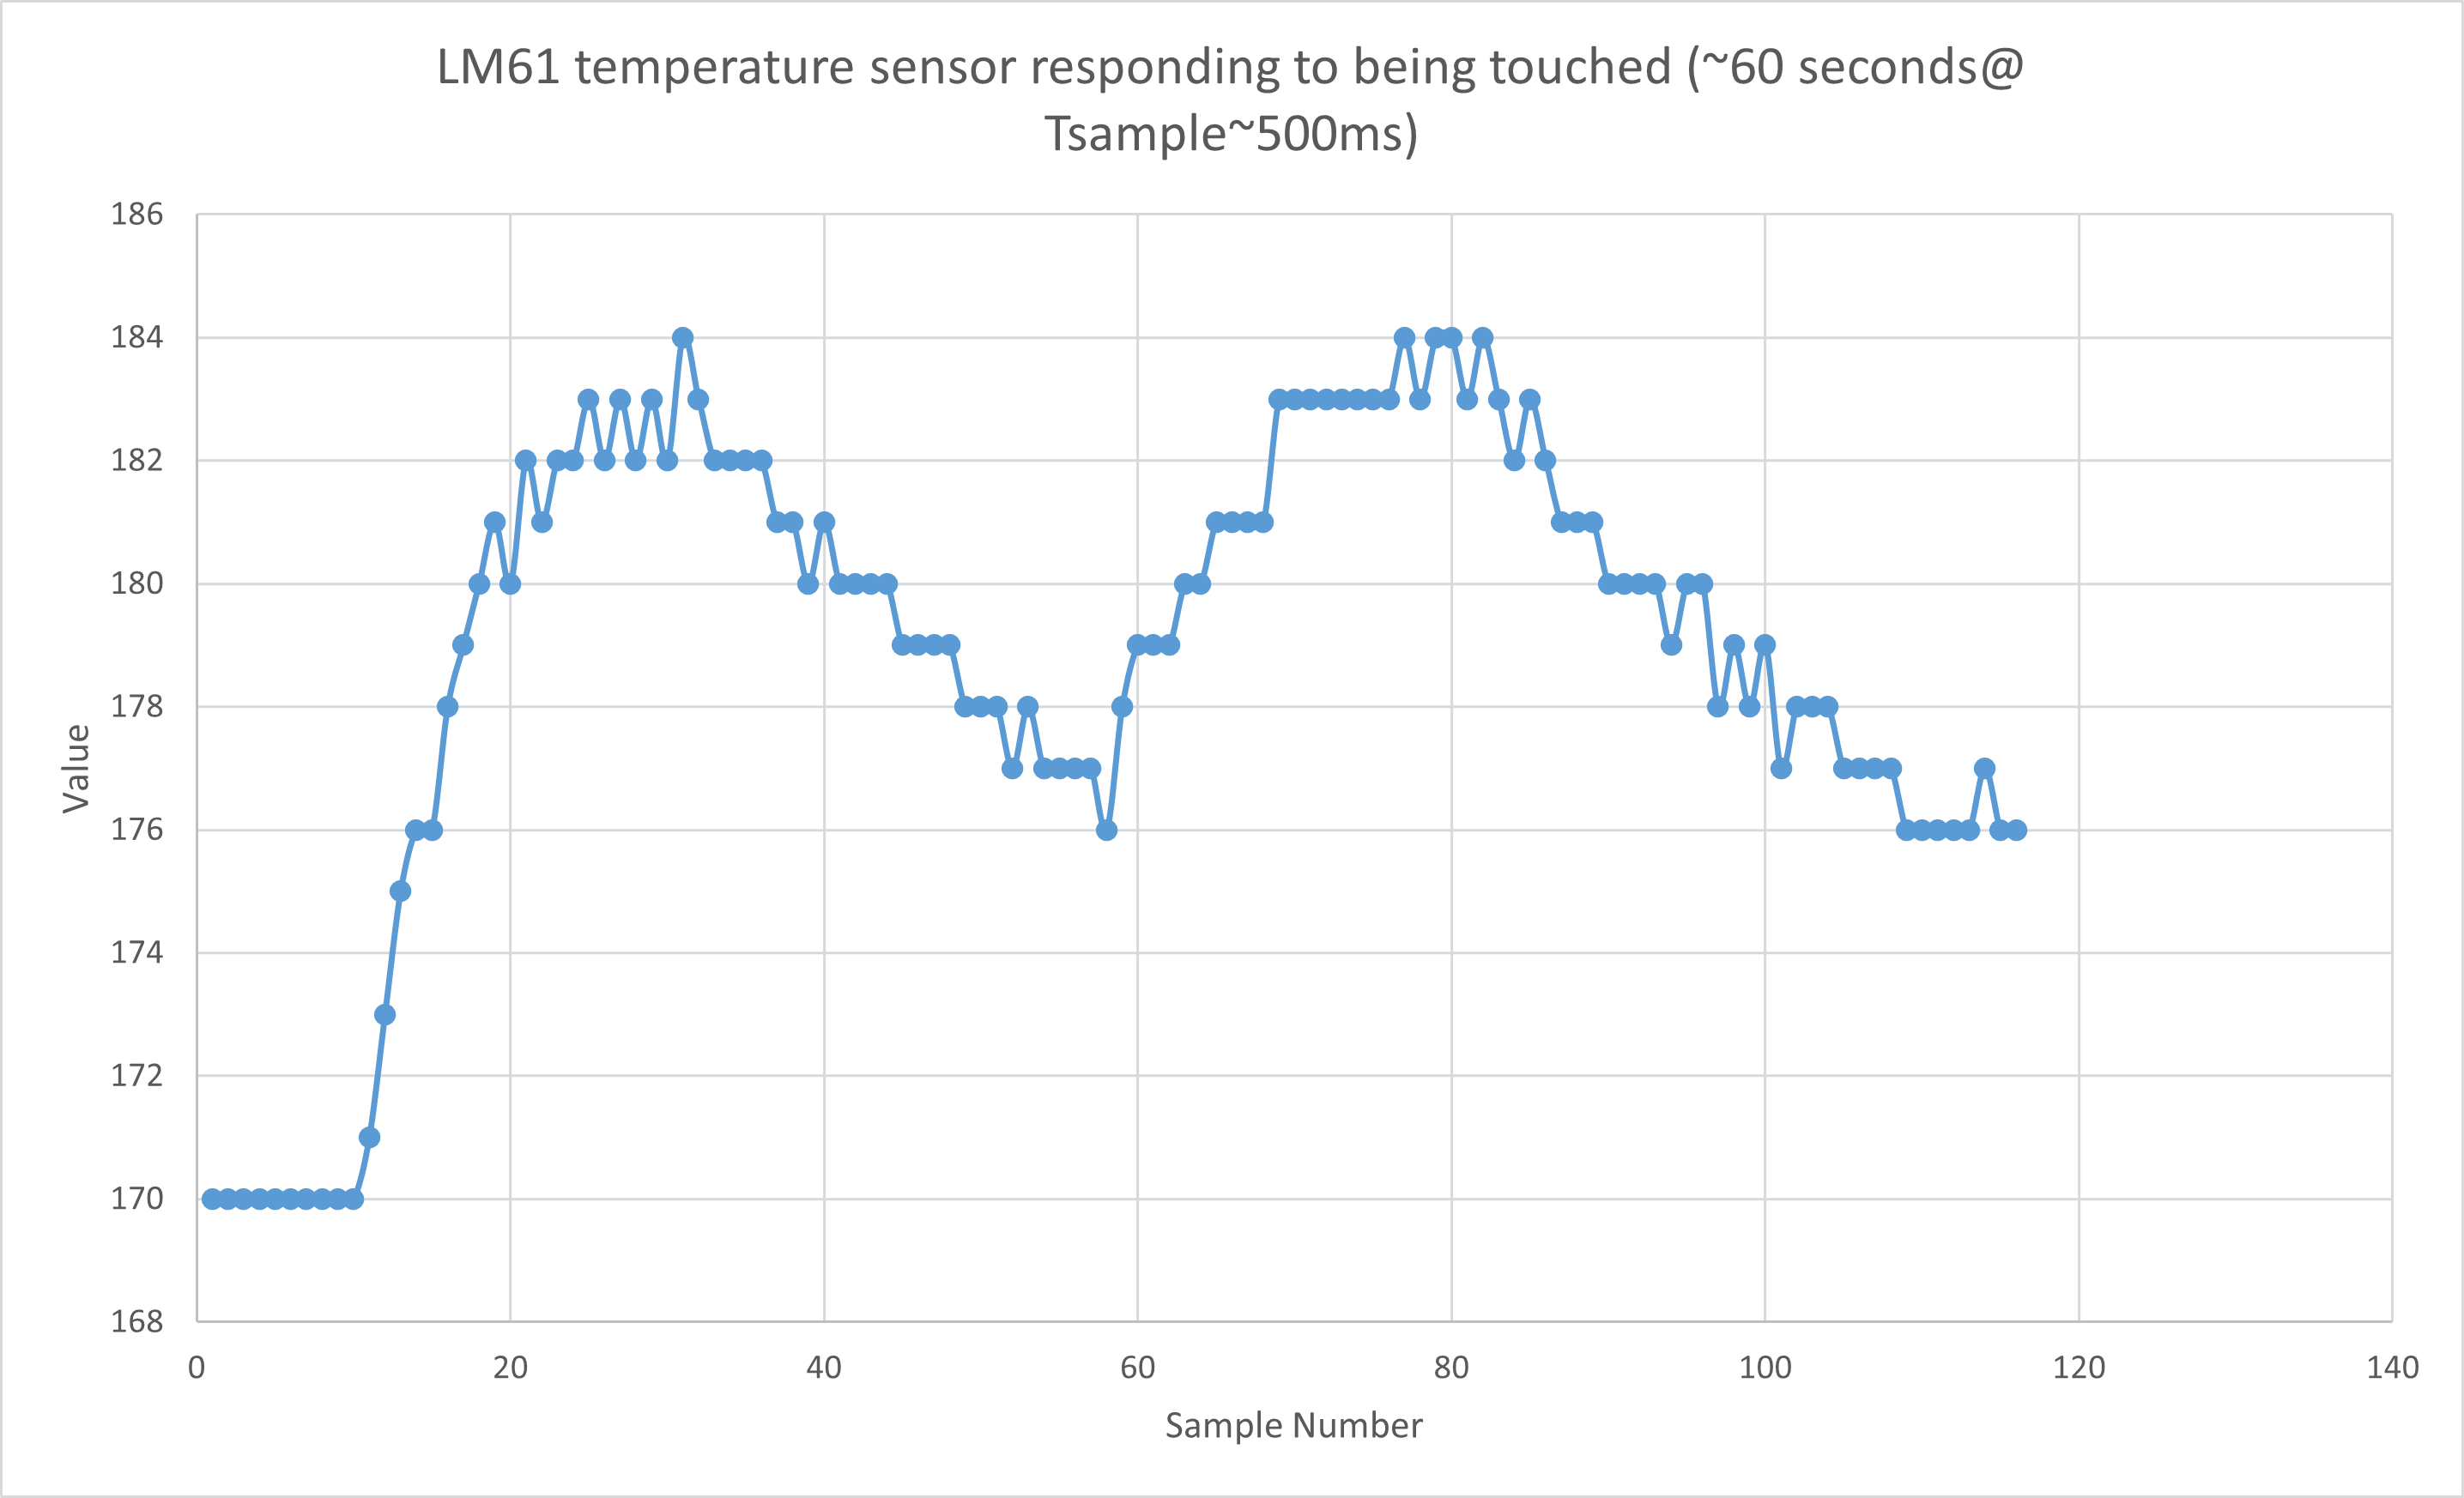
\includegraphics[width=\linewidth]{1.1.png}
    \caption{500 ms Sampling Rate Results}
    \begin{minipage}{\linewidth}
      In this initial setup, the Arduino recorded temperature data at a fixed interval of 500 ms using a hard-coded delay. The results show a smooth progression of temperature values, with minimal fluctuations due to the slow sampling rate.
  \end{minipage}
    \label{fig:part1_500ms}
\end{figure}

%%% Section 2 %%%
\begin{figure}[H]
    \centering
    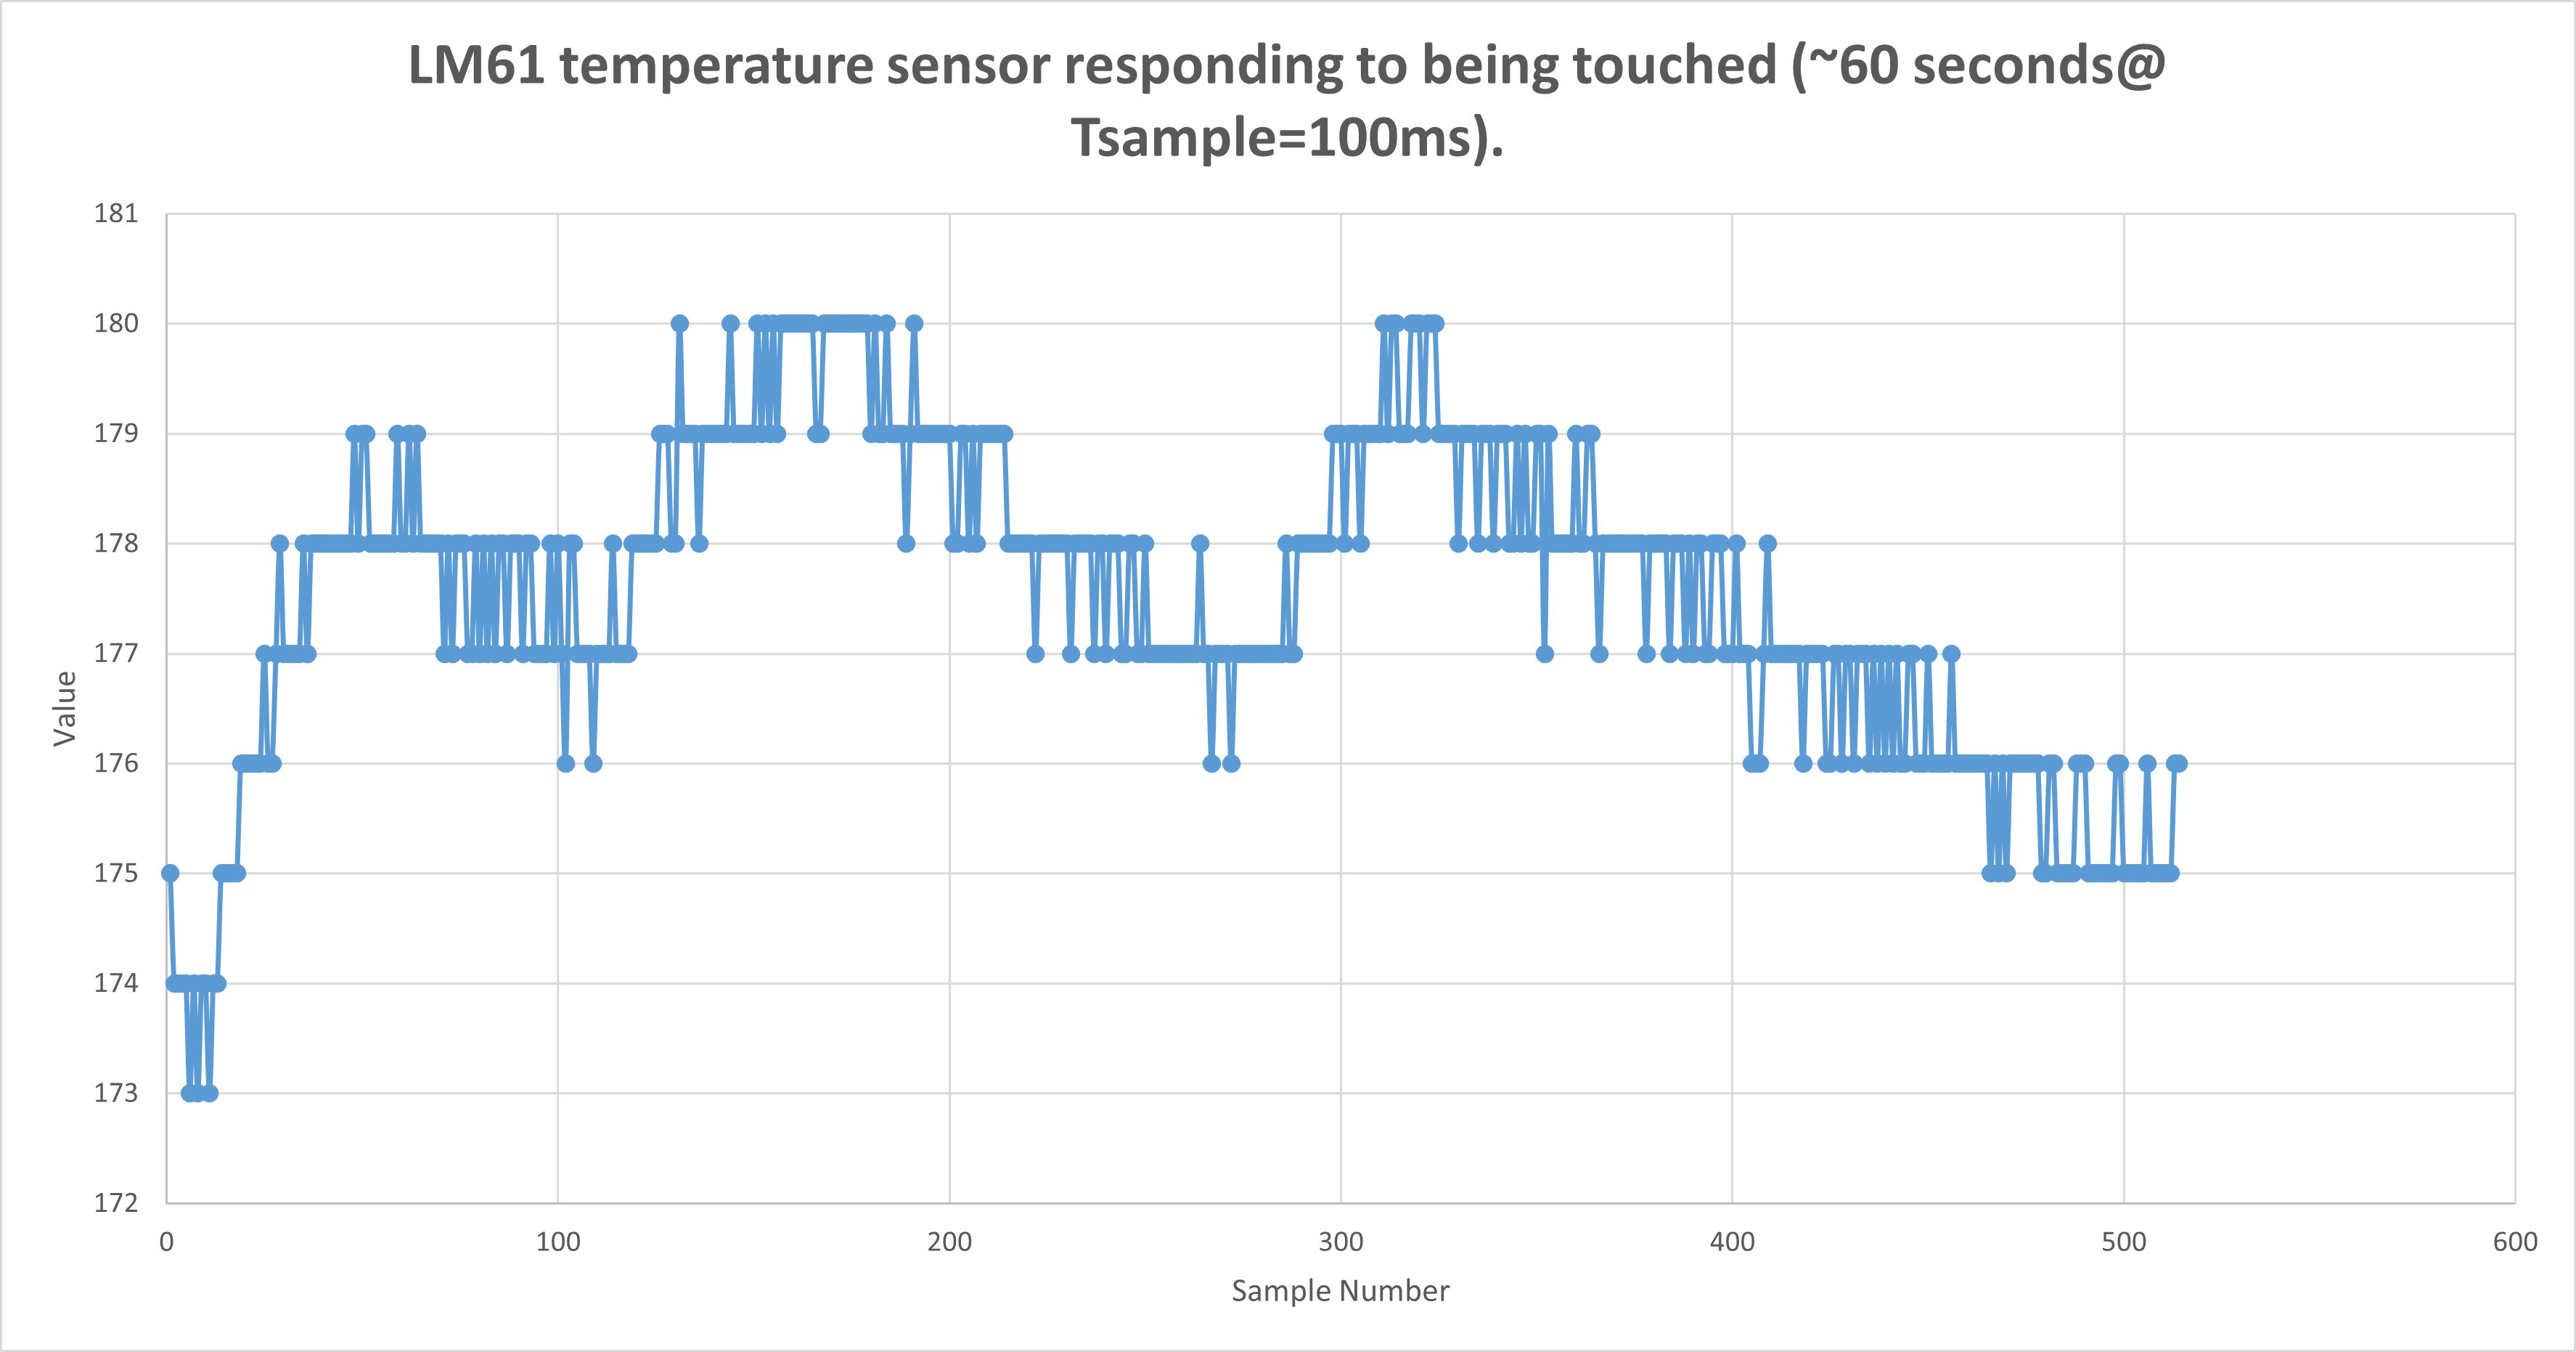
\includegraphics[width=\linewidth]{2.1.png}
    \caption{100 ms Sampling Rate Results}
    \vspace{1em} % Adds vertical space
    \begin{minipage}{\linewidth}
      By replacing the hard-coded delay with a timer interrupt, the sampling rate was increased to 100 ms. The collected data exhibited finer temporal resolution, capturing more details about short-term temperature variations.
    \end{minipage}
    \label{fig:part2_100ms}
\end{figure}

\vspace{-10mm} % Reduce vertical space

%%% Section 3 %%%
\begin{figure}[H]
    \centering
    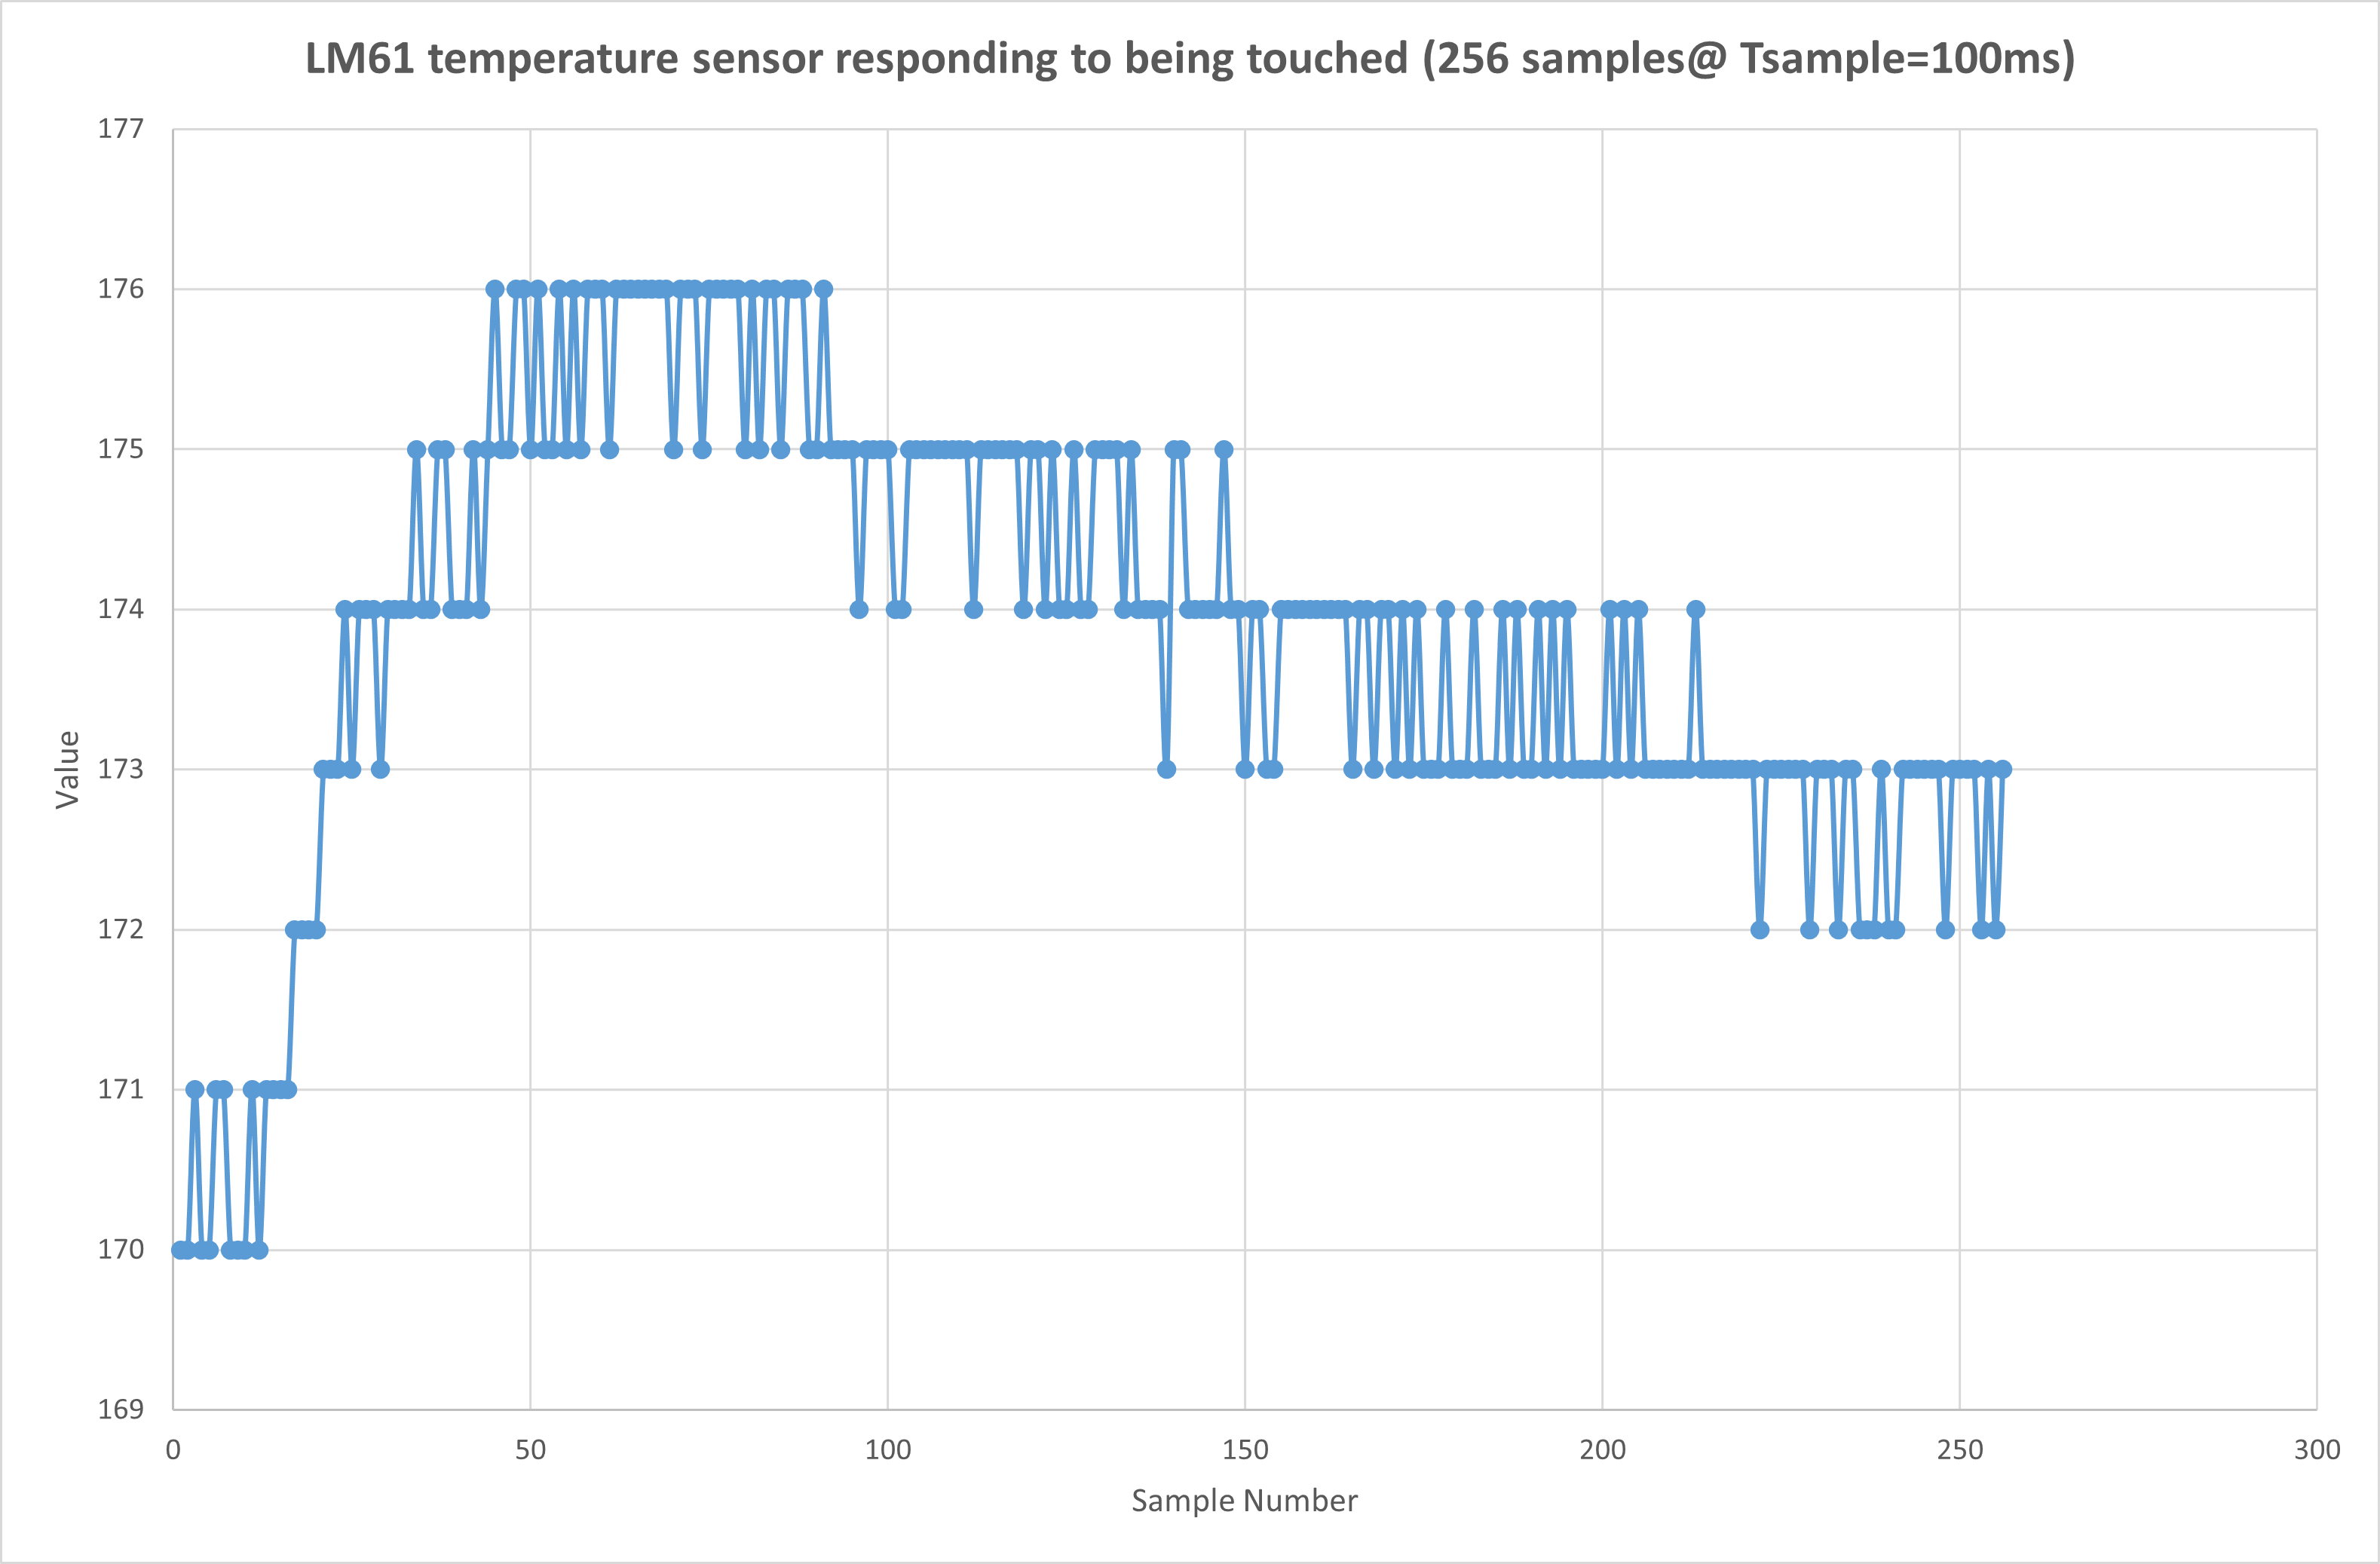
\includegraphics[width=\linewidth]{3.1.png}
    \caption{256 Samples Collected at 100 ms Intervals}
    \begin{minipage}{\linewidth}
      In this iteration, the program was modified to start recording only upon user input and to terminate after collecting 256 samples. This approach ensured consistent data lengths for analysis.
    \end{minipage}
    \label{fig:part3_256_samples}
\end{figure}

\vspace{-10mm} % Reduce vertical space

%%% Section 4 %%%
\begin{figure}[H]
    \centering
    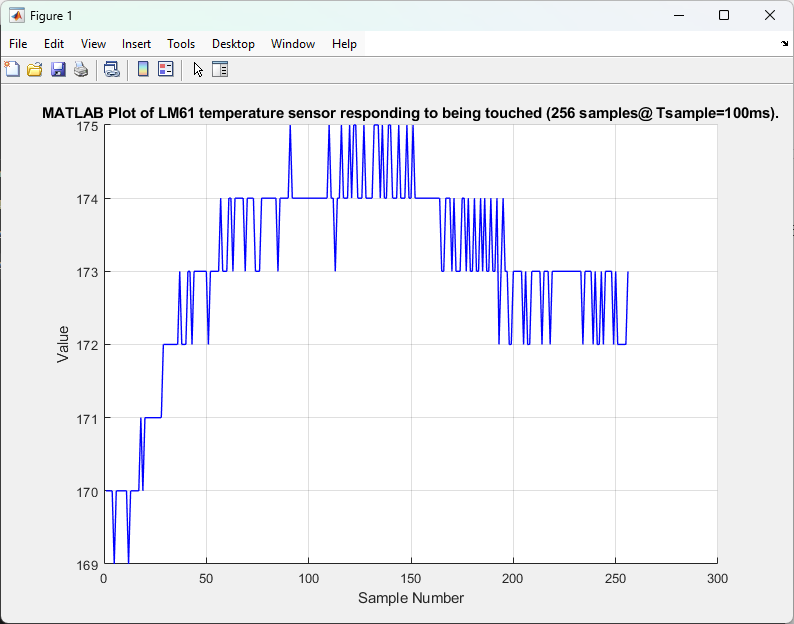
\includegraphics[width=\linewidth]{4.1.png}
    \caption{LM61 Sensor: 256 Samples at 100 ms in MATLAB}
    \begin{minipage}{\linewidth}
      The data collection was integrated with MATLAB, allowing for automated processing and visualization. This setup enabled real-time plotting and streamlined data handling.
    \end{minipage}
    \label{fig:part4_matlab}
\end{figure}

%%% Section 5%%%
Statistical analysis was performed to examine fluctuations in the recorded temperature values. Key metrics such as the mean and standard deviation were computed for different scenarios.

%%% Amplitude Burst %%%
\begin{figure}[H]
    \centering
    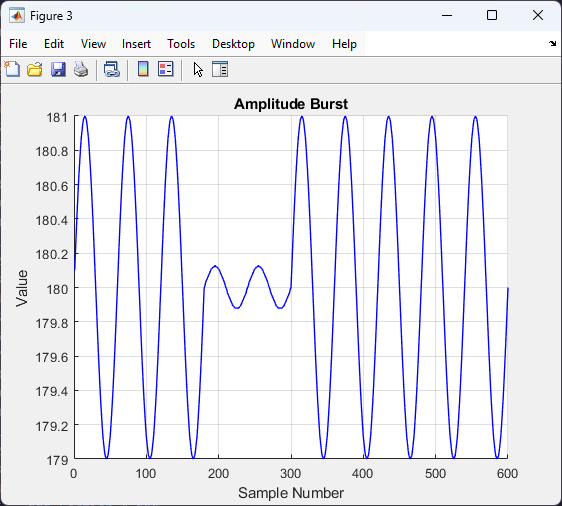
\includegraphics[width=\linewidth]{5.1.1.png}
    \caption{Amplitude Burst Plot}
    \begin{minipage}{\linewidth}
      This test introduced an amplitude burst in the data, simulating abrupt temperature changes. The results show clear deviations in the readings, as illustrated below.
    \end{minipage}
    \label{fig:amplitude_burst}
\end{figure}

\vspace{-10mm} % Reduce vertical space

\begin{figure}[H]
    \centering
    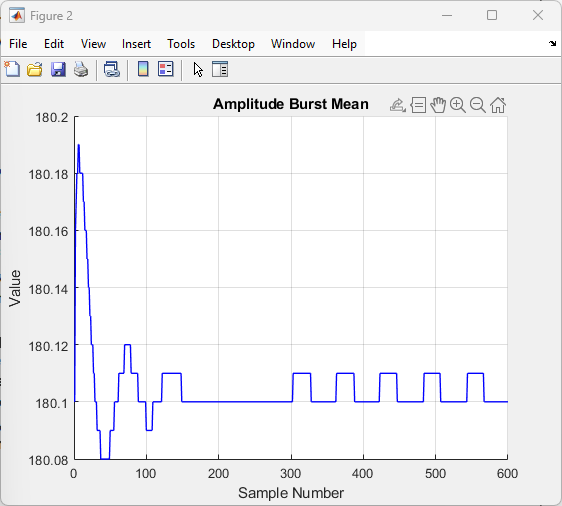
\includegraphics[width=\linewidth]{5.1.2.png}
    \caption{Amplitude Burst Mean}
    \begin{minipage}{\linewidth}
      The calculated mean of the amplitude burst dataset provides insight into the overall temperature shift
    \end{minipage}
    \label{fig:amplitude_burst_mean}
\end{figure}

\vspace{-10mm} % Reduce vertical space

\begin{figure}[H]
    \centering
    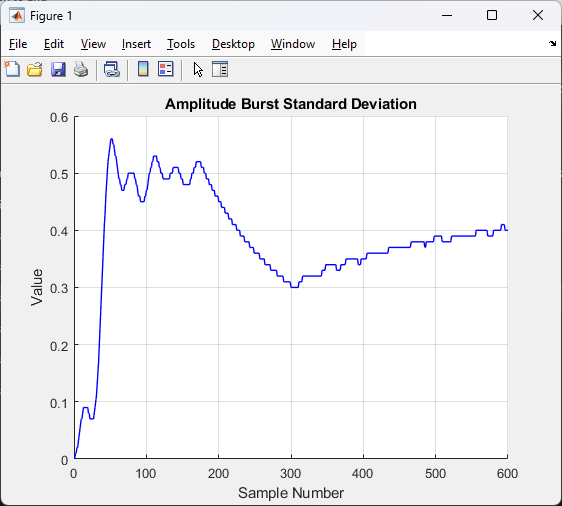
\includegraphics[width=\linewidth]{5.1.3.png}
    \caption{Amplitude Burst Standard Deviation}
    \begin{minipage}{\linewidth}
      The standard deviation plot highlights increased variability during the burst phase.
    \end{minipage}
    \label{fig:amplitude_burst_stddev}
\end{figure}

\vspace{-1em} % Reduce vertical space

%%% Frequency Burst %%%
\begin{figure}[H]
    \centering
    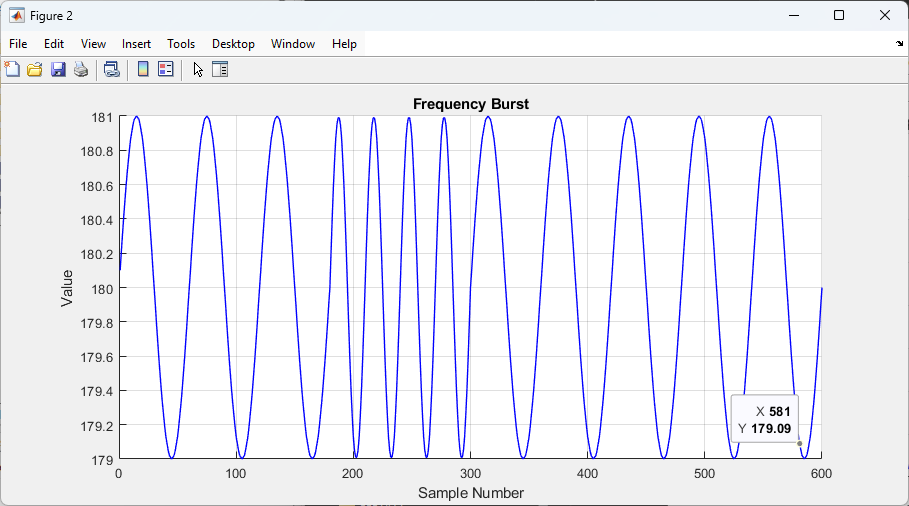
\includegraphics[width=\linewidth]{5.2.1.png}
    \caption{Frequency Burst Plot}
    \begin{minipage}{\linewidth}
      In this case, a frequency burst was introduced, altering the rate of temperature fluctuations. The resulting data captures rapid changes in sensor readings.
    \end{minipage}
    \label{fig:frequency_burst}
\end{figure}

\newpage

\begin{figure}[H]
    \centering
    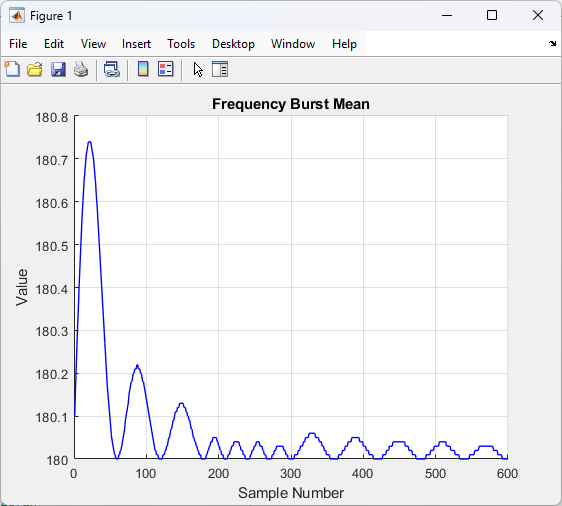
\includegraphics[width=\linewidth]{5.2.2.png}
    \caption{Frequency Burst Mean}
    \begin{minipage}{\linewidth}
      The mean temperature over the frequency burst interval is shown below.
    \end{minipage}
    \label{fig:frequency_burst_mean}
\end{figure}


\begin{figure}[H]
    \centering
    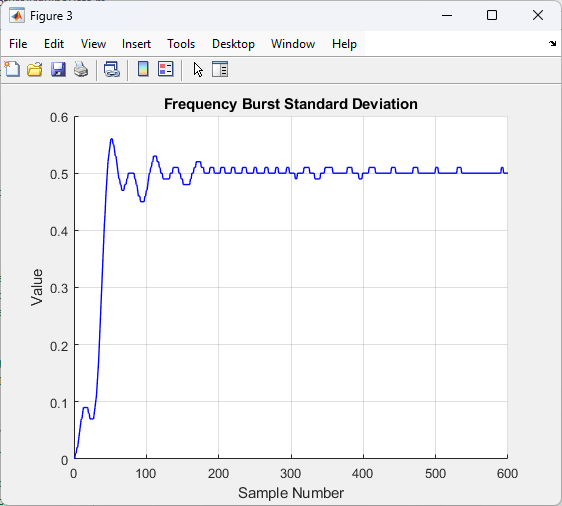
\includegraphics[width=\linewidth]{5.2.3.png}
    \caption{Frequency Burst Standard Deviation}
    \begin{minipage}{\linewidth}
      The standard deviation plot indicates increased variation due to the burst.
    \end{minipage}
    \label{fig:frequency_burst_stddev}
\end{figure}

\section{Analysis}
The analysis of mean and standard deviation in statistics is crucial, as these variables are indicators of the procedure's success. For P1-5 the Arduino code was edited to calculate the mean and standard deviation of the samples. \par

The standard deviation is more responsive to temperature variations than the mean because it captures the extent of changes in the data, where the mean only provides a central value. The formula for standard deviation accounts for the squared differences between each data point and the mean, making it more sensitive to larger deviations. In contrast, the mean smooths out variations by averaging all values, reducing the impact of extreme temperature changes. For instance, if temperature readings fluctuate significantly over time, the standard deviation will increase, reflecting the variation, while the mean may remain relatively stable. This makes standard deviation a better indicator of dynamic temperature changes.

\section{Conclusion}
The experimental setup successfully demonstrated an optimized method for temperature data collection using an Arduino and IC system. By progressively improving data recording techniques, the lab highlighted the advantages of interrupt-based sampling, user-controlled initiation, and MATLAB integration for enhanced data analysis. The statistical evaluation reinforced the reliability of the collected data and provided deeper insights into temperature changes.

Future work could explore additional enhancements such as adaptive sampling rates, machine learning-based anomaly detection, and integration with wireless communication for remote data monitoring. These improvements would further increase the system’s versatility and applicability in real-world temperature monitoring scenarios.

\end{document}